\section{Diseño (Desarrollo Teórico)}
\subsection{Diagrama a bloques del sistema}
En la siguiente figura, se muestra el diagrama a bloques del sistema, donde se destaca que es lo que
conforma cada una de las partes de potencia, microprocesador, comunicación y periféricos.
\begin{figure}[htp]
    \centering
    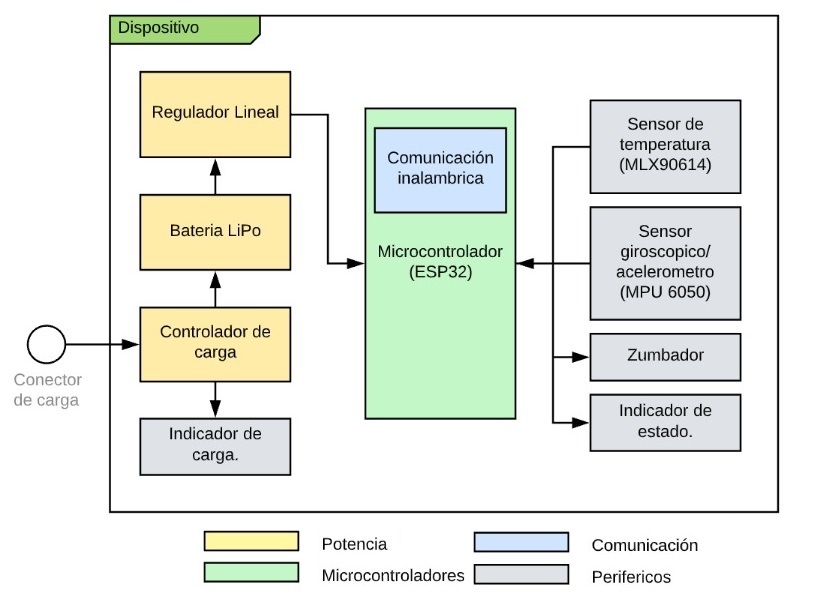
\includegraphics[width=\columnwidth]{system_block_diagram.png}
    \caption{Diagrama a bloques del sistema.}
\end{figure}

\subsection{ESP32}
ESP32 es la denominación de una familia de chips SoC de bajo costo y consumo de energía, con tecnología Wi-Fi
y Bluetooth de modo dual integrada. El ESP32 emplea un microprocesador Tensilica Xtensa LX6 en sus variantes
de simple y doble núcleo e incluye interruptores de antena, balun de radiofrecuencia, amplificador de potencia,
amplificador receptor de bajo ruido, filtros, y módulos de administración de energía. El ESP32 fue creado y
desarrollado por Espressif Systems y es fabricado por TSMC utilizando su proceso de 40 nm.

\subsubsection{Características}
\begin{itemize}
    \item Procesador:
          \begin{itemize}
              \item CPU: microprocesador de 32-bit Xtensa LX6 de doble núcleo (o de un solo núcleo), operando a 160 MHz.
              \item Co-procesador de ultra baja energía (ULP).
          \end{itemize}
    \item Memoria: 520 KiB SRAM
    \item Conectividad inalámbrica:
          \begin{itemize}
              \item Wi-Fi: 802.11 b/g/n
              \item Bluetooth: v4.2 BR/EDR y BLE
          \end{itemize}
    \item Interfaces periféricas:
          \begin{itemize}
              \item 2 × interfaces I²C
              \item 3 × UART
          \end{itemize}
    \item Administración de energía:
          \begin{itemize}
              \item Regulador interno de baja caída
              \item Corriente de 5µA en modo de suspensión profundo
          \end{itemize}
\end{itemize}

\begin{figure}[htp!]
    \centering
    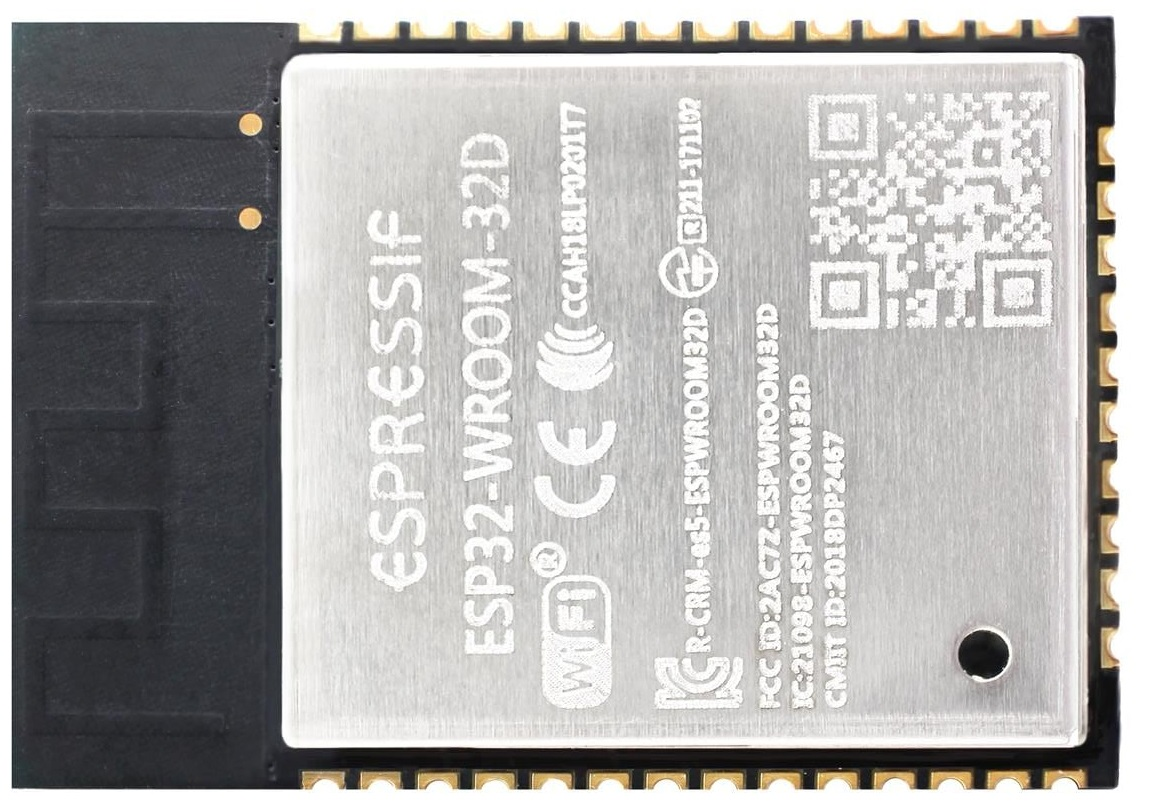
\includegraphics[width = 0.25 \textwidth]{ESP32-WROOM-32D_t.jpg}
    \caption{ESP32 WROOM.}
    \label{fig: esp32}
\end{figure}
\FloatBarrier

\subsubsection{Comparativa}
Despues de realizar las pruebas se encontró que el ESP32 cuenta con buena eficiencia para realizar operaciones, además de una gran ventaja frente a los otros microcontroladores al contar con la comunicación Bluetooth y wifi integrada.

A continuación se muestran los resultados comparados de las pruebas al realizar operaciones con punto flotante.
\begin{figure}[htp!]
    \centering
    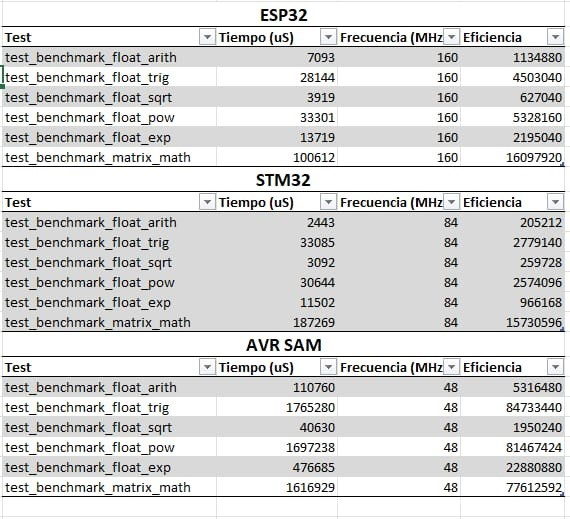
\includegraphics[width=0.35\textwidth]{benchmark_table_esp32.jpg}
    \caption{Tabla comparativa de los microcontroladores propuestos.}
    \label{fig: table_benchmark}
\end{figure}
\FloatBarrier

\begin{figure}[htp!]
    \centering
    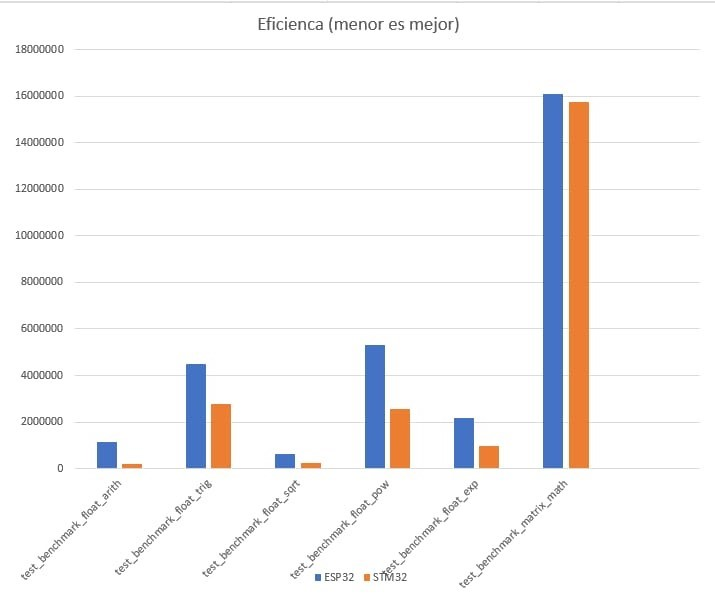
\includegraphics[width=\columnwidth]{benchmark_graphic_esp32.jpg}
    \caption{Grafica comparativa ESP32.}
    \label{fig: graphic_benchmark}
\end{figure}
\FloatBarrier

\subsection{Sensores}
\subsubsection{MPU-9250}
El MPU-9250 de InvenSense, es un \acrshort{imu} de 9 ejes, que combina
un giroscopio de 3 ejes, un acelerómetro de 3 ejes, y un magnetómetro de 3 ejes, donde cada
uno de estos cuenta con:
\begin{itemize}
    \item Tres \acrshort{adc} de 16 bits para digitalizar sus salidas.
    \item Registros individuales de configuración, ya sea para rangos, frecuencia de muestreo, habilitación, etc.
\end{itemize}

La union de estos tres sensores y sus posibles configuraciones permiten el desarrollo de sistemas de detección/medición de
movimientos con una buena fiabilidad.

\begin{figure}[htp]
    \centering
    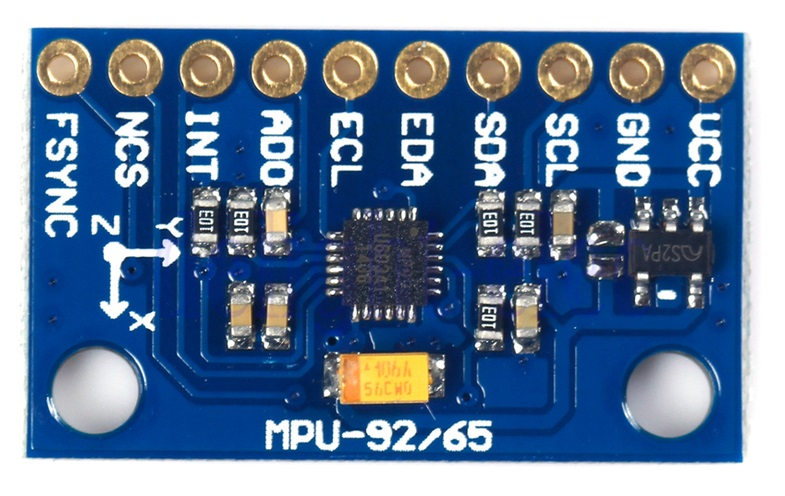
\includegraphics[ width = 0.27 \textwidth  ]{mpu_9250_board.png}
    \caption{MPU-9250. }
\end{figure}

\paragraph{Caracteristicas}
\begin{itemize}
    \item Giroscopio de tres ejes de salida digital con un rango de escala completa programable de $\pm250$, $\pm500$, $\pm1000$ y $\pm\SI{2000}{\radian\per\second}$.
    \item Acelerómetro de tres ejes de salida digital con un rango de escala completa programable de $\pm2g$, $\pm4g$, $\pm8g$ y $\pm16g$.
    \item Sensor magnético monolítico de efecto Hall de 3 ejes con concentrador magnético con resolución de 0,6T/\acrshort{lsb}.
    \item Cuenta con interfaz para comunicación por \acrshort{spi} y \acrshort{i2c}.
\end{itemize}

\subsubsection{Sensor de temperatura infrarrojo MLX90614}
El Sensor de temperatura infrarrojo permite medir la temperatura de un objeto a distancia (sin contacto).
El Sensor MLX90614 es un chip de silicio con una fina membrana micro mecanizada, diseñada para ser sensible
a la radiación infrarroja emitida por un objeto a distancia. El sensor posee internamente una etapa de
amplificación y conversión analógica-digital de la señal procedente de la membrana. La salida del sensor es lineal
y se compensa de acuerdo con las variaciones de la temperatura ambiente.

El sensor MLX90614 integra un circuito de filtrado de ruido, un \acrshort{adc} de 17 bits de resolución
y un procesador digital de señales, entregando un amplio rango de trabajo para objetos desde -70°C hasta
380°C, con una precisión de 0.5°C.

\begin{figure}[htp!]
    \centering
    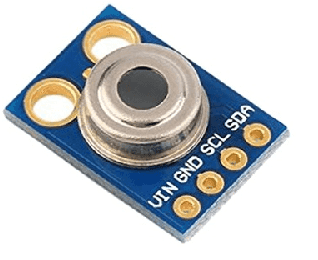
\includegraphics[width = 0.25 \textwidth]{mlx90614_board.png}
    \caption{Sensor MLX90614.}
    \label{fig: sensor}
\end{figure}\FloatBarrier

\paragraph{Caracteristicas}
\begin{itemize}
    \item Voltaje de operación: 3.3V-5V \acrshort{dc}
    \item Protocolo de comunicación \acrshort{smbus} (subconjunto del \acrshort{i2c})
    \item Precisión: $ \pm $0.5°C
    \item \acrshort{adc} interno de 17 bits
    \item Procesador digital de señal interno
    \item Regulador de voltaje 3.3V en placa
    \item Resistencias Pull-up a VIN en placa
\end{itemize}

\subsection{Comunicación}
    \subsubsection{Bluetooth Low Energy}
    Es una tecnología de red de área personal inalámbrica, diseñada y comercializada por Bluetooth SIG
    destinada a aplicaciones en el cuidado de la salud, fitness y beacons,1 seguridad y las industrias
    de entretenimiento en el hogar Comparado con Bluetooth clásico, Bluetooth Low Energy está diseñado
    para proporcionar un bajo consumo de energía, manteniendo un rango de alcance de comunicación similar.

    Los sistemas operativos móviles, incluidos iOS, Android, Windows Phone y BlackBerry, así como macOS,
    Linux, Windows 8 y Windows 10, son compatibles con Bluetooth Low Energy. Bluetooth SIG predice que
    el 100\% de los dispositivos con Bluetooth comercializados hasta 2024 soportaran Bluetooth Low Energy.

    \paragraph{Características}
    \begin{itemize}
        \item Permite la comunicación entre dispositivos de pila de botón y dispositivos.
        \item Bluetooth, que opera en 2.4 GHz (una de las bandas ISM), con una tasa de transferencia de 1 Mbps en la capa física.
        \item Los chips de \acrshort{ble} tienen amplias opciones de empleo en la industria.
        \item Tienen el mismo tamaño de los dispositivos Bluetooth clásicos.
        \item Tiene soporte para seguridad, ya que emplean el sistema de cifrado AES y esquemas de seguridad configurables.
    \end{itemize}

    \begin{figure}[htp!]
        \centering
        
\includegraphics[width = 0.30 \textwidth]{bluetooth.png}
        \caption{Logotipo de \acrshort{ble}.}
        \label{fig: bluetooth}
    \end{figure}
    \FloatBarrier

\subsection{Aplicación Movil}
    \subsubsection{Flutter}    
    Flutter es un \acrshort{sdk} para el de código fuente abierto de desarrollo de aplicaciones móviles creado por Google 
    para el lenguaje de programación Dart. Suele usarse para desarrollar interfaces de usuario para aplicaciones en Android, iOS y Web 
    así como método primario para crear aplicaciones para Google Fuchsia.​

    \begin{figure}[htp!]
        \centering
        
\includegraphics[width = 0.30 \textwidth]{flutter.png}
        \caption{Logotipo de Flutter.}
        \label{fig: flutter}
    \end{figure}
    \FloatBarrier

